\documentclass[a4paper,12pt]{report}
\usepackage{float, amsmath, bm, graphicx, numprint, multicol, caption}

\begin{document}

\setlength{\abovedisplayskip}{6pt}
\setlength{\belowdisplayskip}{8pt}
\setlength{\abovedisplayshortskip}{2pt}
\setlength{\belowdisplayshortskip}{8pt}

\title{Project 2 Report}
\author{Dylan Callaway}
\date{Engineering 150 \\ Fall 2019}
\maketitle

\pagenumbering{roman}
\tableofcontents
\newpage
\pagenumbering{arabic}

\newenvironment{nscenter}
 {\setlength{\topsep}{0ex}\trivlist\item\relax\centering}
 {\endtrivlist}

\section{Introduction}
The scenario being modeled in this project is that of 15 unmanned aerial vehicles (UAVs) that navigate through a three-dimensional (3D) field of 25 randomly placed obstacles in order to map the location of 100 randomly placed targets. The UAVs motion is governed by physical laws and several control equations. The aim of this project is to determine the optimal parameters of the control equations using a genetic algorithm to perform the optimization.

This paper will provide an introduction to the physical laws, control algorithm, and the optimization method used. It will then outline the procedure for running the simulation, as well as any pertinent results that followed.


\section{Background and Theory}
The dynamics of each of the UAVs is modeled using the following relationships in a 3D, fixed Cartesian coordinate system where $x_i$ is some state variable of the $i^{th}$ agent (denoted by the subscript $i$).

\subsection{Physical Laws}
The kinematics of the UAVs can be expressed as a function of the kinetics in the following manner\footnote{State variables without the $0$ superscript vary over time as in $x_i(t)$. However, $(t)$ is left out for brevity.}:
$$\bm{a}_i = \frac{\bm{\Psi}^{tot}_i}{m_i} \qquad \qquad \bm{\Psi}^{tot}_i = \bm{F}^d_i +\bm{F}^p_i$$
is the total force, $m_i$ is the mass, and $\bm{a}_i$ is the resultant acceleration. $\bm{F}^d_i$, the drag force, is a function of $\bm{v}_i$, the velocity, and $\bm{F}^p_i$, the propulsive force, is a function of the control algorithm outlined in the following section.
 
The position, $\bm{r}_i$, and the velocity, $\bm{v}_i$, can be determined for each UAV according to the definitions of position, velocity, and acceleration in Cartesian coordinates and the UAV's initial conditions, expressed as $\bm{v}_i^0$ and $\bm{r}_i^0$ for velocity and position, respectively.
$$\bm{v}_i = \bm{v}_i^0 + \int_{0}^{t}{\bm{a}_i dt} \qquad \bm{r}_i = \bm{r}_i^0 + \int_{0}^{t}{\bm{v}_i dt}$$

These equations are numerically integrated during the simulation using Forward Euler time discretization, such that they become:
$$\bm{v}_i(t+\Delta t) = \bm{v} _i(t) + \bm{a}_i(t)\Delta t \qquad \bm{r}_i(t+\Delta t) = \bm{r}_i(t) + \bm{v}_i(t)\Delta t$$

where some state variable $\bm{x}_i(t)$ is that state variable at the current time step, and $\bm{x}_i(t+\Delta t)$ is that state variable at the next time step.

The Forward Euler method for discretizing this system is a good choice as it relies minimally on computing intermediate values to determine the new states. This makes it simple to encode and generally fast to compute on desktop hardware. However, this method does have a few drawbacks, mainly relating to the size of $\Delta t$.

If $\Delta t$ is too large, the entirety of the function may not be captured. This is because the slope of the function at the given time step is extrapolated from that time for $\Delta t$. So, if the function changes slope at all during that $\Delta t$, it would be impossible for this method of integration to capture that.

Furthermore, any error that occurs as a result of the above phenomenon will be added to any and all previous errors. This can create problems in simulations that are meant to emulate physical reality, because the solution will be further from reality the longer it runs.

Both of these inaccuracies can be improved on by reducing the size of $\Delta t$, however this comes at the cost of increased computation time, sometimes to such an extent that it is not practical to reduce $\Delta t$ any further. In this project, that was not an issue, and a $\Delta t$ of $.2s$ yielded acceptable results.

A key simplifying assumption used in this project is that each UAV can be modeled sufficiently as a point mass. There are two primary things that must be true for this assumption to be valid. First, the distance covered by the UAVs must be much larger than the UAVs themselves, such that their true form does not significantly affect their path. And second, the UAVs must be sufficiently rigid that their intra-body dynamics do not affect their inter-body dynamics significantly. Both of these criteria are true in the scope of this project.

Another assumption used is that the affects of gravity, lift, and buoyancy are negligible relative to the affects of the propulsive force on the UAVs. This simplifies the problem from an encoding and computational standpoint, and allows the UAVs to perform the task more effectively. Adding gravity, for example, would require the propulsive force vector (which has a fixed magnitude) to have a greater upward component, thereby limiting acceleration in that direction and thus the ability to avoid obstacles and map targets. The other forces, lift and buoyancy, can be thought of as having similar effects.
 
\subsection{Control Algorithm}
As shown in the previous section, the acceleration of the UAVs is determined in part by $\bm{F}^p_i$, which is defined as follows:
$$\bm{F}^p_i = F^p_i\bm{n}^*_i$$
where $F^p_i$ is a constant scalar and $\bm{n}^*_i$ is a unit vector determined by the control algorithm explained here.

For each $i^{th}$ UAV the Euclidean distance is calculated to each $j^{th}$ other UAV, target, or obstacle according to the following, where $x \in \{m, t, o\}$, respectively:
$$\bm{d}^{mx}_{ij} = \bm{r}_i - \bm{r}^x_j$$
$$d^{mx}_{ij} = ||\bm{d}^{mx}_{ij}|| = \sqrt{(r_{i,1} - r^x_{j,1})^2 + (r_{i,2} - r^x_{j,2})^2 + (r_{i,3} - r^x_{j,3})^2}$$
The unit vector from the $i^{th}$ UAV and $j^{th}$ UAV, target, or obstacle is then:
$$\bm{n}^{mx}_{ij} = \frac{\bm{d}^{mx}_{ij}}{d^{mx}_{ij}}$$
From $d^{mx}_{ij}$ and $\bm{n}^{mx}_{ij}$ the interaction vector, $\hat{\bm{n}}^{mx}_{ij}$, can be determined:
$$\hat{\bm{n}}^{mx}_{ij} = \bm{n}^{mx}_{ij} (\eta^{mx}_{ij} - \epsilon^{mx}_{ij})$$
$$\eta^{mx}_{ij} = w_{x, 1}e^{-q_1d^{mx}_{ij}} \qquad \epsilon^{mx}_{ij} = w_{x, 2}e^{-q_2d^{mx}_{ij}}$$
where $\eta^{mx}_{ij}$ is the attraction term and $\epsilon^{mx}_{ij}$ is the repulsion term. Once $\hat{\bm{n}}^{mx}_{ij}$ is determined for each $x \in \{m, t, o\}$, the total interaction vector for the $i^{th}$ UAV and each other UAV, target, or obstacle is calculated according to:
$$\bm{N}^{mm}_i = \sum_{j=1, j\neq i}^{N_m}\hat{\bm{n}}_{ij}^{mm} \qquad \bm{N}^{mt}_i = \sum_{j=1}^{N_t}\hat{\bm{n}}_{ij}^{mt} \qquad \bm{N}^{mo}_i = \sum_{j=1}^{N_o}\hat{\bm{n}}_{ij}^{mo}$$
Adding the interaction vectors for the other UAVs, targets, and obstacles with the following weights produces the total interaction vector for the $i^{th}$ UAV as follows:
$$ \bm{N}^{tot}_i = W_{mm}\bm{N}^{mm}_i + W_{mt}\bm{N}^{mt}_i + W_{mo}\bm{N}^{mo}_i $$
The direction of the propulsion force for the $i^{th}$ UAV is then given by:
$$  \bm{n}^*_i = \frac{\bm{N}^{tot}_i}{||\bm{N}^{tot}_i||} $$
This completes the determination of $\bm{F}_i^p$ which affects the UAVs motion by being fed back into the physical laws shown in the previous section.

\section{Procedure and Methods}
\subsection{Optimization Parameters}
There were several parameters in the control algorithm that were left undefined in the previous section. These parameters are scalar values in the range $[0, 2]$. The goal of the optimization is to find parameters that allow the UAVs to map as many targets as possible, with as few crashes as possible, in as short a time as possible. In order to perform the optimization, these goals are translated into the following cost function:
$$\Pi = w_1M^* + w_2T^* + w_3L^* \qquad w_1 = 70 \quad w_2 = 10 \quad w_3 = 20$$
$$ M^* = \frac{(Unmapped\ targets)}{(Total\ targets)} \qquad T^* = \frac{(Used\ time)}{(Max\ time)} \qquad L^* = \frac{(Crashed\ UAVs)}{(Initial\ UAVs)}$$
This cost function provides feedback on the key parameters of the problem, and weighs them in a logical way, wherein mapping the targets is the primary goal. Targets are mapped if they are within a specified distance of a UAV. UAVs crash if they exit a specified area, or if they are within a specified distance of an obstacle or another UAV. This function is also easily tune-able if, for example, the UAVs were expensive and you did not want to lose any of them due to crashing you could increase the weight placed on $L^*$. 

This type of problem, which by inspection can be seen to have several local extrema, is not well suited to being solved by gradient based methods which may converge to said local extrema instead of the global minima. It may be possible to use a broader search method, like grid search, and then perform gradient based optimization, but that takes significantly longer then a genetic algorithm like that used here. The genetic algorithm is a good choice because it simultaneously searches a large solution space, while converging to an optimal solution. In problems with many design variables, 15 in this case, that drastically reduces the time required to compute a solution compared to methods that do these steps one after the other.

The control model implemented in this problem adds weight to the attraction or repulsion of a UAV from another object proportional to the exponential of the distance and some scalar weight. This is a commonly used control method for simple systems, and can be observed to provide good results in a number of applications. There is no rigorous physics based proof that demonstrates its applicability versus other similar methods, but it can be seen in the dynamics of many physical systems that their behavior over time approaches that of a decaying exponential function.

A critical aspect of the aforementioned model is that it is a \textit{decaying} exponential. Thus meaning the power term must be negative. If the power the exponential is raised to were to become positive, two things will happen that will negatively affect the performance of the UAVs. First, the output of the exponential will not be constrained to $[0, 1]$, and second the interaction between the UAV and other objects will increase with distance, rather than decrease. This means that the UAVs would have strong reactions to objects that they have no chance at mapping or crashing into any time soon, but may miss nearby mappable targets or crash right into nearby obstacles, without reacting in any meaningful way beforehand.

In this implementation of the simulation, the mapped targets and crashed UAVs are removed from the existing group by setting their coordinates to NaN. This simulation was done in MATLAB, so the NaN specification allows two key things. First, the mapped targets or crashed agents can be easily located with the function isnan(). Second, by using isnan(), all of the state variables of a given UAV or target (position, velocity, distance to to other objects, etc) can also be set to NaN. Originally, the mapped targets and crashed UAVs were removed from their respective arrays. However, this created a challenge in keeping track of the other arrays of state variables that also needed that UAV or target to be removed. The downside to doing it using NaN is that the array maintains its size and the NaN must be set to 0 during summation, in order to preserve the rest of the data (summing NaN always returns NaN in MATLAB). Both of these drawbacks add computational time but it is not significant.

There are many ways to place the agents that yield good results. Ultimately, the agents ended up being place is a vertical grid on the -X side of the simulation area. This positioned them far enough from eachother so as to not crash or interact too intensely and increased the likelihood that they did not all move to the same targets.

\section{Results and Discussion}
\begin{figure}[H]
\begin{nscenter}
  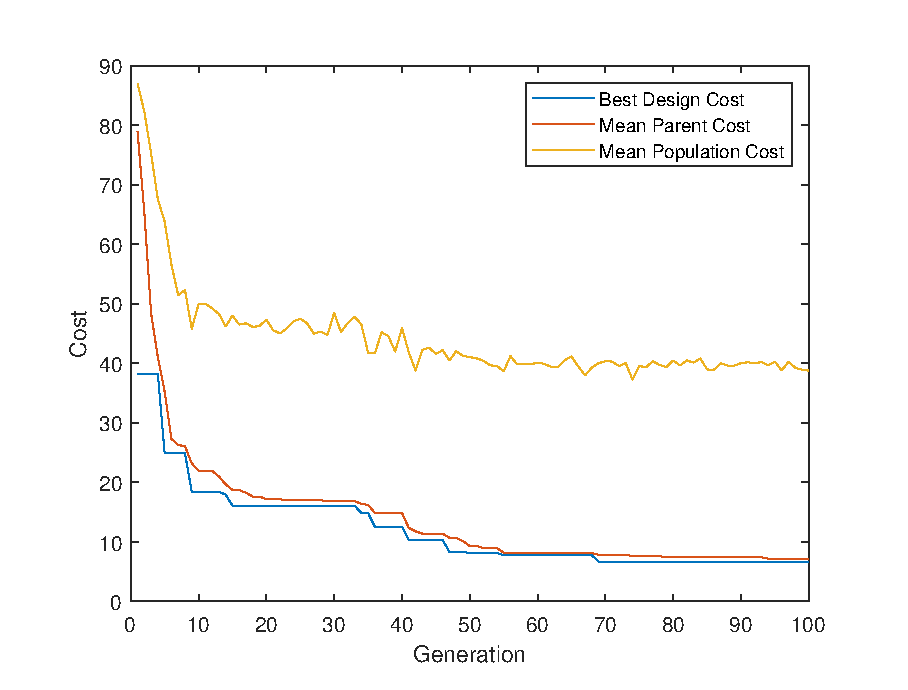
\includegraphics[width=0.5\linewidth]{results1.eps}
  \caption{Various Weighted Costs vs. Generation.}
  \end{nscenter}
\end{figure}
Figure 1 shows the cost of the best design from the genetic algorithm converging to about 7. Most of the parent designs have a cost of a similar value. Something interesting to note is that after about 25 generations, the overall population cost is relatively constant. This is because once the parents are all optimal, they no longer continually reduce the overall average cost, and the other designs for each generation are simply random.
\begin{figure}[H]
\begin{nscenter}
  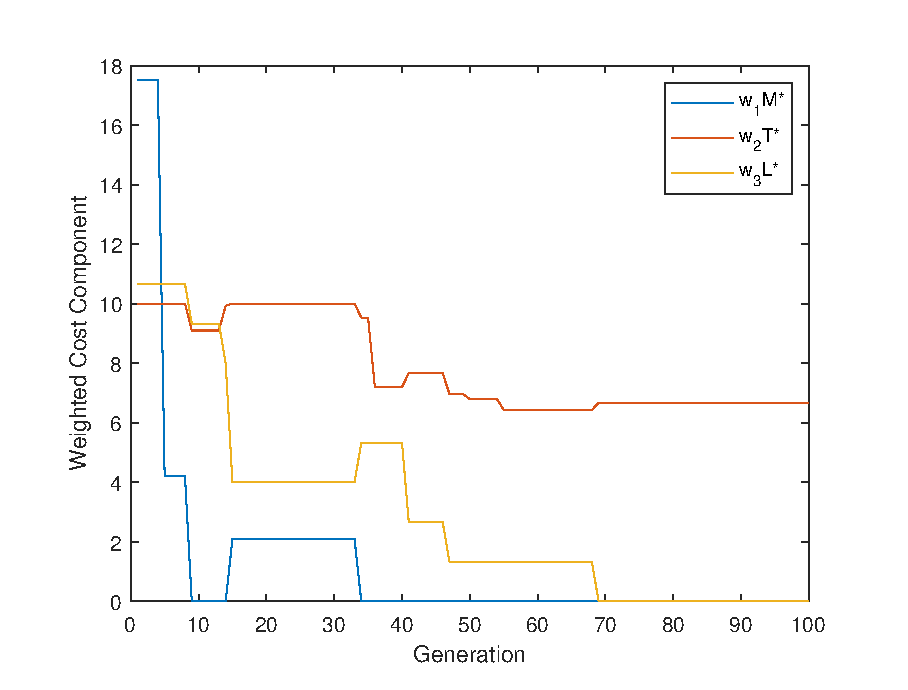
\includegraphics[width=0.5\linewidth]{results2a.eps}
  \caption{Best Weighted Design Cost Component vs. Generation.}
    \end{nscenter}
\end{figure}
\noindent
An interesting thing to note in Figure 2 is that $w_1M^*$ drops the most quickly. This is because $w_1 = 70$ while the other two weights are less than half of that, causing $M^*$ to really drive the optimization. There are even some iterations where $w_2T^*$ or $w_3L^*$ increase while $w_1M^*$ decreases with the overall cost decreasing.
\begin{figure}[H]
\begin{nscenter}
  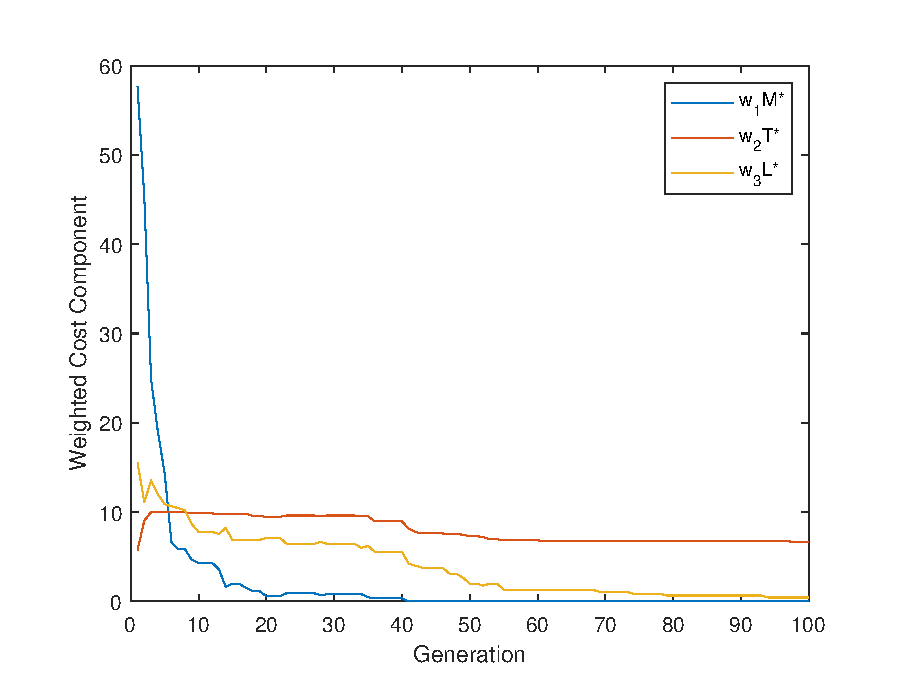
\includegraphics[width=0.5\linewidth]{results2b.eps}
  \caption{Mean Parental Weighted Design Cost Component vs. Generation.}
    \end{nscenter}
\end{figure}
\noindent
Figure 3 demonstrates a similar phenomena as Figure 2, with $w_1m^*$ again decreasing most sharply for the parent designs. In plain English it can be thought of as the genetic algorithm selecting parents first for things that prevents $M^*$ increasing, and then after that is largely taken care of, worrying about the other traits of a given design. This is evidenced by the fact that $w_3L^*$ continues to decrease up to the $100^{th}$ generation. $w_1M^*$ and $w_2T^*$ have essentially converged to their final values by generation 40 or 50, but $w_3L^*$ continues to decrease and the parameters made more optimal. $L^*$ is the fraction of agents that have crashed, and $w_3 = 20$ is greater than $w_3$, but less than $w_1$, so it is interesting that altering the parameters causes this cost component to continually fall while the others are constant.
\begin{figure}[H]
\begin{nscenter}
  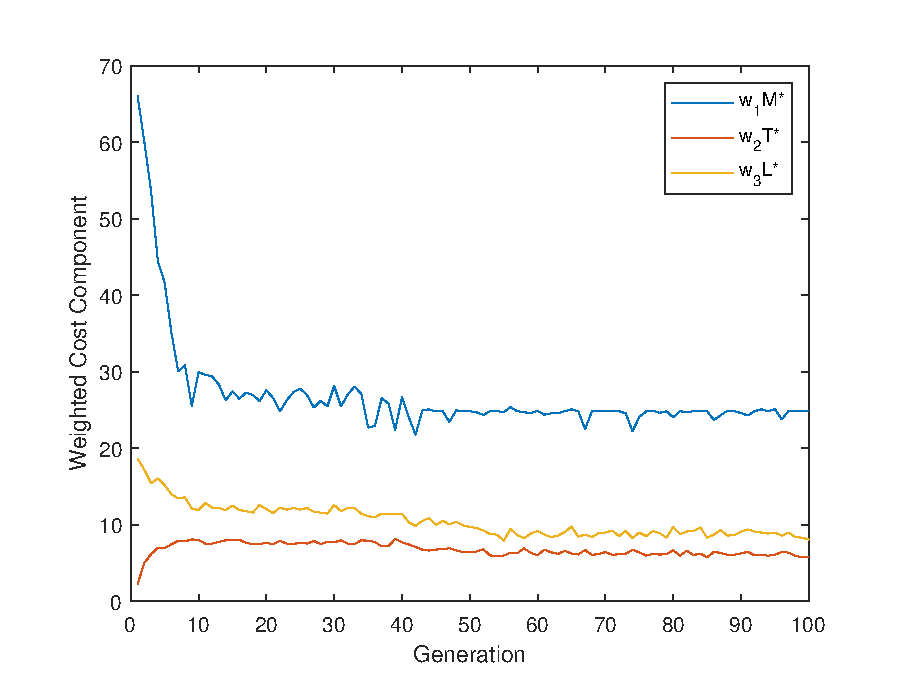
\includegraphics[width=0.5\linewidth]{results2c.eps}
  \caption{Mean Overall Weighted Design Cost Component vs. Generation.}
    \end{nscenter}
\end{figure}
\noindent
Like in Figure 1, once the parents have essentially converged, the overall population cost is relatively high and constant due to most of the population being random at that point, and few random guesses being more optimal than the already highly optimized parents.

\begin{table}[H]
\caption{Design Parameters and Cost of the Best Designs}
\resizebox{\textwidth}{!}{
\begin{tabular}{c|c|c|c|c|c|c|c|c|c|c|c|c|c|c|c|c}
 Design & $\Pi$ & $\Lambda_1$ & $\Lambda_2$ & $\Lambda_3$ & $\Lambda_4$ & $\Lambda_5$ & $\Lambda_6 $& $\Lambda_7 $& $\Lambda_8$& $\Lambda_9$& $\Lambda_{10}$& $\Lambda_{11}$& $\Lambda_{12}$& $\Lambda_{13}$& $\Lambda_{14}$& $\Lambda_{15}$ \\ 
 \hline
 \hline
1 & 6.667 & 1.388 & 0.268 & 1.435 & 0.757 & 0.735 & 0.214 & 0.485 & 0.740 & 0.878 & 0.089 & 1.655 & 1.864 & 0.674 & 1.003 & 0.267   \\  
 
2 & 6.733 & 1.389 & 0.277 & 1.435 & 0.761 & 0.742 & 0.215 & 0.486 & 0.740 & 0.882 & 0.092 & 1.648 & 1.863 & 0.673 & 1.003 & 0.273   \\  
 
3 & 6.733 & 1.388 & 0.272 & 1.435 & 0.759 & 0.738 & 0.214 & 0.486 & 0.740 & 0.879 & 0.090 & 1.652 & 1.864 & 0.674 & 1.003 & 0.270  \\  
 
4 & 7.067 & 1.389 & 0.275 & 1.435 & 0.760 & 0.741 & 0.214 & 0.486 & 0.740 & 0.881 & 0.091 & 1.650 & 1.863 & 0.674 & 1.003 & 0.272 \\  
\end{tabular}
}
\end{table}

\noindent
As can be seen in Table 1, there is very little variation in the parameters of the top four designs. None of the parameters are negative because the genetic algorithm only searches on the interval $[0, 2]$. Some of the parameters are nearly 0, and some are nearly 2. For these values, setting the near 0 ones to 0, and increasing the interval for the ones near 2 may yield better performance, as that seems like what the simulations wants, anyways.

\pagebreak
Below is a series of plots of the UAV swarm 8 seconds apart, each. The first is the starting formation, and the last is the formation right as the final target is mapped.

\begin{figure}[H]
\minipage{0.5\textwidth}
  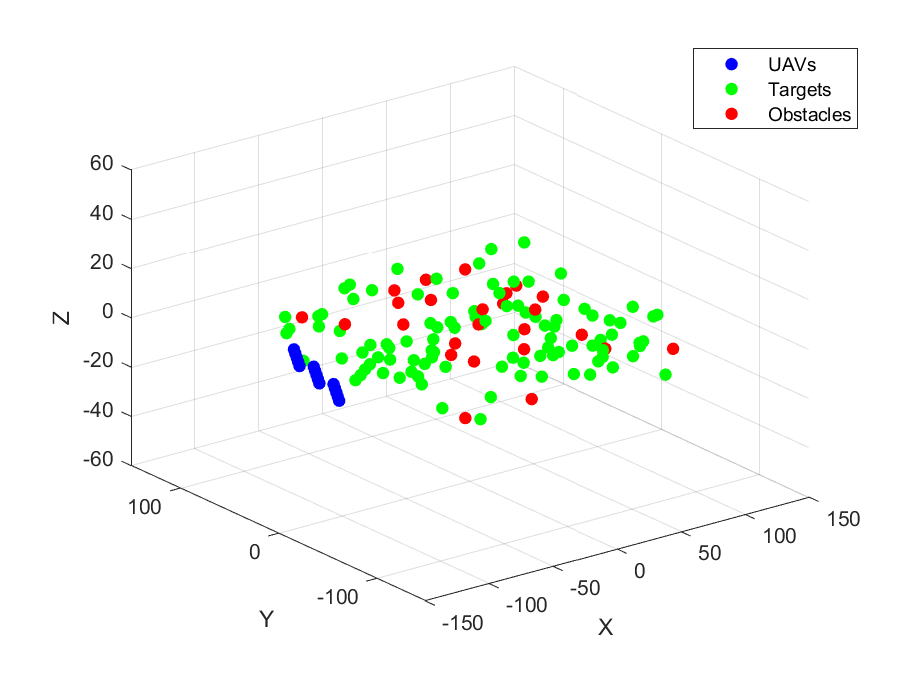
\includegraphics[width=\linewidth]{uav0.eps}
  \caption{UAV swarm at $t = 0$.}
    \endminipage\hfill
  \minipage{0.5\textwidth}
  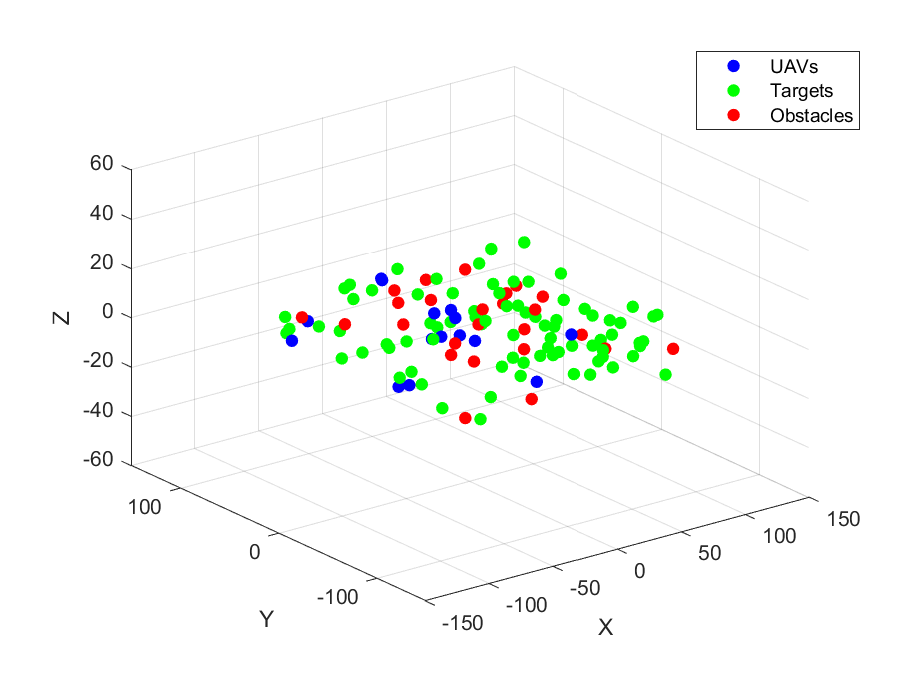
\includegraphics[width=\linewidth]{uav40.eps}
  \caption{UAV swarm at $t = 8$.}
    \endminipage\hfill
  \minipage{0.5\textwidth}
  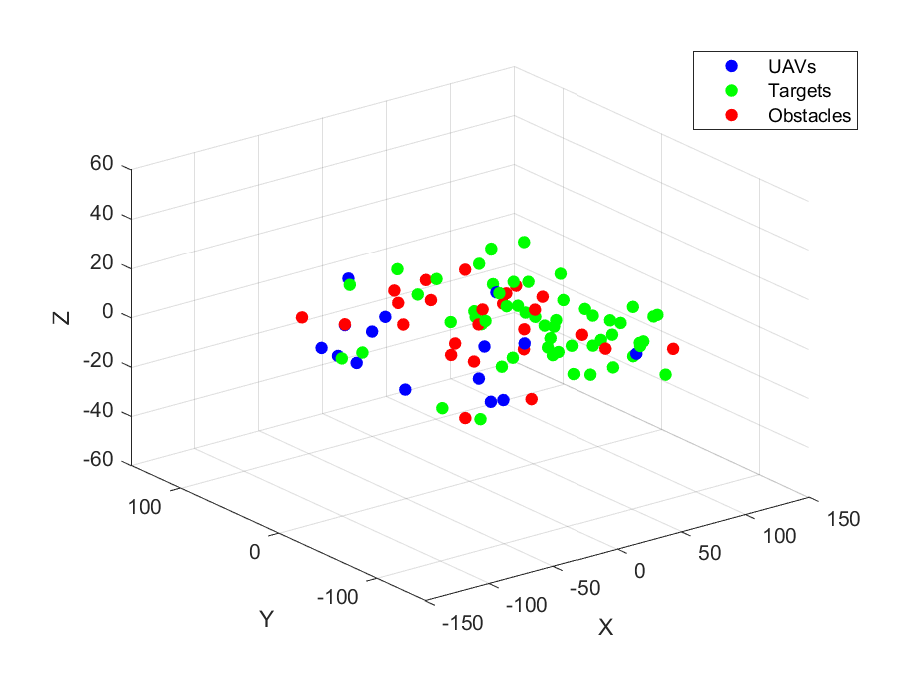
\includegraphics[width=\linewidth]{uav80.eps}
  \caption{UAV swarm at $t = 16$.}
    \endminipage\hfill
  \minipage{0.5\textwidth}
  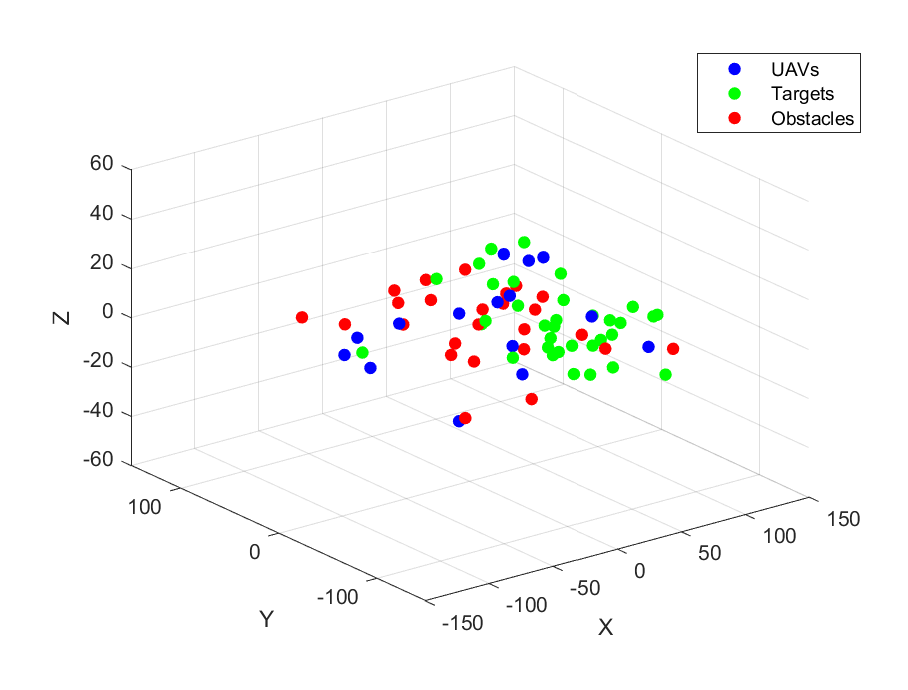
\includegraphics[width=\linewidth]{uav120.eps}
  \caption{UAV swarm at $t = 24$.}
    \endminipage\hfill
  \minipage{0.5\textwidth}
  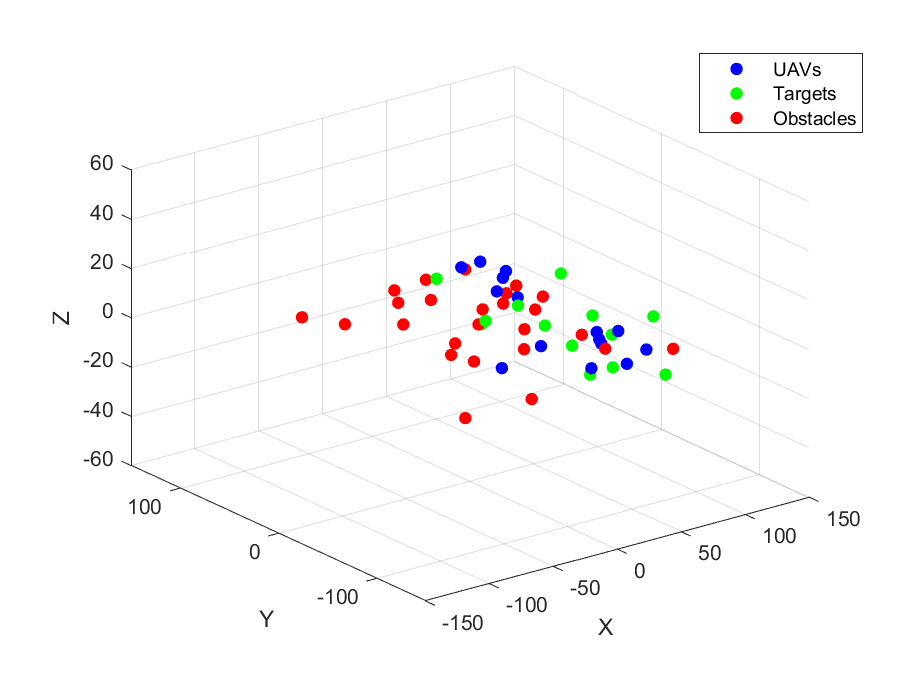
\includegraphics[width=\linewidth]{uav160.eps}
  \caption{UAV swarm at $t = 32$.}
    \endminipage\hfill
  \minipage{0.5\textwidth}
  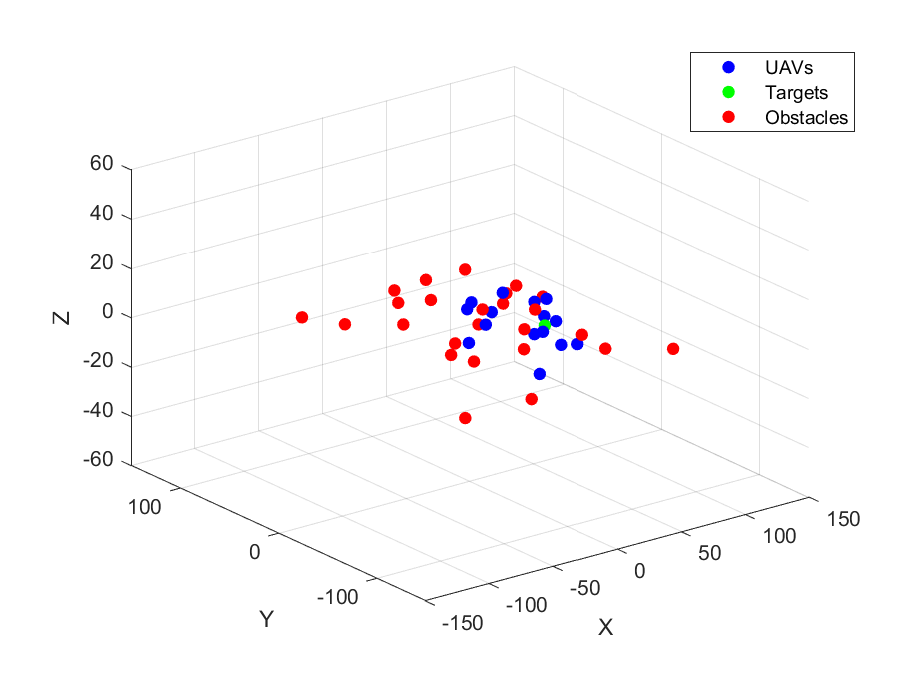
\includegraphics[width=\linewidth]{uav200.eps}
  \caption{UAV swarm at $t = 40$.}
    \endminipage
\end{figure}

\section{Conclusion}
This project aimed to find optimal parameters for UAV swarm target mapping. The dynamics of the UAVs was modeled and integrated using the Forward Euler method, a control algorithm with exponentially decaying influence on drone motion with respect to Euclidean distance was implemented, and a genetic algorithm was used to perform the optimization of said control algorithm's parameters. The final result is a set of control parameters that allow the mapping to be carried out with zero loss of UAVs, 100\% of targets mapped, and a final run time of only 40 seconds.

\section{Appendix}
Appendix is empty.



\end{document}